\documentclass[final,hyperref={pdfpagelabels=false}]{beamer}
\mode<presentation>
{
	%  \usetheme{Berlin}
	\usetheme{Dreuw}
}
\usepackage{times}
\usepackage{amsmath,amsthm, amssymb, latexsym}
\boldmath
\usepackage[english]{babel}
\usepackage[latin1]{inputenc}
\usepackage[orientation=portrait,size=a0,scale=1.4,debug]{beamerposter}

%%%%%%%%%%%%%%%%%%%%%%%%%%%%%%%%%%%%%%%%%%%%%%%%%%%%%%%%%%%%%%%%%%%%%%%%%%%%%%%%%5
\graphicspath{./Concordialogo.jpg}
\title[ProjectName]{Scientific Calculator: Power Function f(x) = $x^y$}
\author[AuthorName]{Sanchit Kumar (40081187)}
\institute[UniversityName]{Concordia University, SOEN 6011 - Software Engineering Processes}
\date{\today}


%%%%%%%%%%%%%%%%%%%%%%%%%%%%%%%%%%%%%%%%%%%%%%%%%%%%%%%%%%%%%%%%%%%%%%%%%%%%%%%%%5
\begin{document}
	\begin{frame}{} 
		
		\begin{block}{\Large Introduction}
			{\large A power function is of the form: f(x) = $x^y$ ,where y is a real number.}\par \vspace{1.5cm}
			
			\textbf{Maclaurin \& Taylor Series}
			\begin{equation} \label{exptaylor}
				e^x = 1 + \frac{x}{1!} + \frac{x^2}{2!}  + \frac{x^3}{3!} + \frac{x^4}{4!} ...... \frac{x^n}{n!}
			\end{equation}
			
			\begin{equation} \label{logtaylor}
			\ln{\frac{1+x}{1-x}} = 2 * ( \frac{x}{1} + \frac{x^3}{3} + \frac{x^5}{5} + \frac{x^7}{7}  .....)
			\end{equation}
			
			\textbf{\large{Critical Scenarios}}
			\begin{itemize}
				\item $0^y$ where $y \leq 0$, is undefined.
				\item $x^y$ where $x < 0$ and $y = m/n$ and n is even, is undefined.
			\end{itemize}
			
			\vspace{1cm}
			\textbf{\large{Functional Requirememts}}
			\begin{enumerate}
				\item System should prompt the user to enter the value of x and y.
				\item System should display an error message when value entered by user is not a number.
				\item In case the input entered is not valid system should prompt the user to input values again. 
				\item User should have the option to exit the program anytime during the use.
				\item System should display an error message when user enter value of x and y both as 0.
				\item System should display an error message when user enter value of x as 0 and y as a negative number.
			\end{enumerate}
			
			
			\textbf{\large{Non-Functional Requirememts}}
			\begin{enumerate}
				\item The error message displayed should be appropriate and helpful for the user. 
				\item The result displayed should be as accurate as possible.
				\item Calculation time should be less than 1 second.
			\end{enumerate}
			
		\end{block} 
		
		

		\begin{columns}[t]
			
			\begin{column}{.48\linewidth}
				\begin{block}{\Large Process Flow}
					\hspace{2cm} 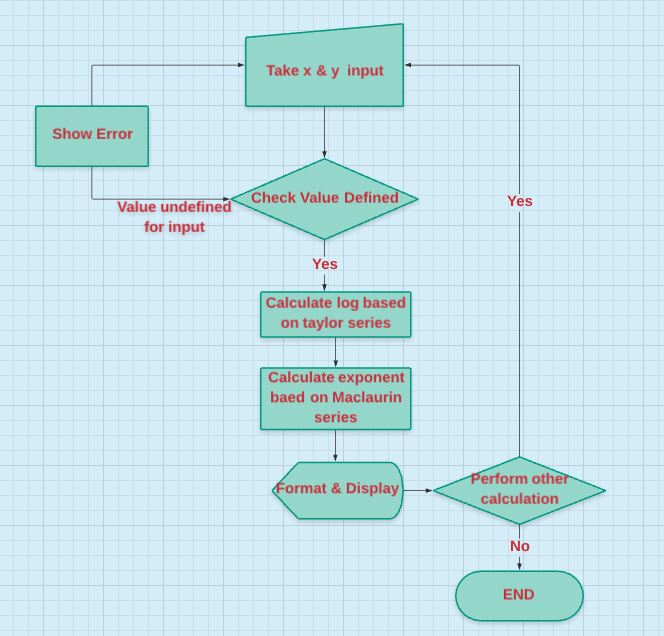
\includegraphics[width=30cm, height=20cm]{Flow.JPG}
				\end{block}
			\end{column}
			\begin{column}{.48\linewidth}
				\begin{block}{\Large Application UI: Text-based}
					\hspace{1cm} 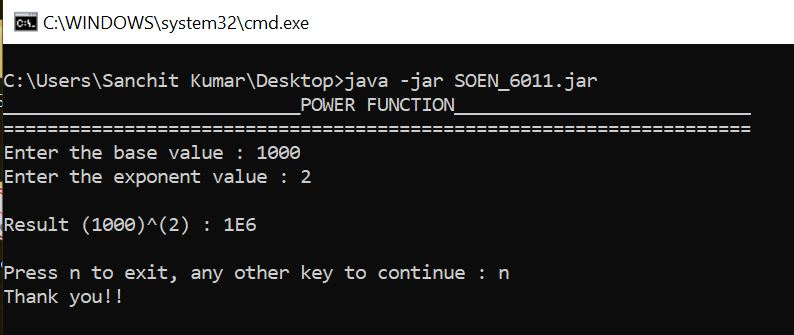
\includegraphics[width=35cm, height=20cm]{UI.JPG}
				\end{block}
			\end{column}
			
		\end{columns}

		
		\begin{block}{\Large Technical Specifications}
			\textbf{\large Risk Identified during Prototype Design} \\ \vspace{0.5cm}
			\begin{itemize}
				\item Use of double and float data types can pose risk because of possible loss of precision by using such data type. For this purpose we need BigDecimal Data Type.
				\item Need to be aware of typecasting when casting int, float or double to BigDecimal. Such conversions may not be highly accurate and can result in loss of precision.
			\end{itemize}

			\vspace{1cm}			
			\textbf{\large Development Environment} \\ \vspace{0.5cm}
			\begin{itemize}
				\item \textbf{IDE: }IntelliJ IDEA, \textbf{Development Language: }Java, \textbf{Testing Framework: }JUnit5
				\item \textbf{Debugger: }IntelliJ Built-in Debugger, \textbf{Source Code Analysis: }IntelliJ Upsource
			\end{itemize}
			
		\end{block}
	
		\begin{block}{\Large Learnings}
			\textbf{\large Critical Decisions Made} \\ \vspace{0.5cm}
			\begin{itemize}
					\item Use of BigDecimal Data type. Why? To get highly precise answers as expected in case of a scientific calculator, use of BigDecimal or BigInteger is preferable rather than float or double. However, special care should be taken for explicit or implicit type conversions when working with BigDecimal.
			\end{itemize}
		
		\vspace{0.5cm}
		\textbf{\large Lessons Learnt} \\ \vspace{0.5cm}
		\begin{itemize}
			\item Through this project I realised the importance of prototyping and its valuable use in risk reduction and addressing the problem at an early stage of development. Also, prototyping helped me to reduce development time and cost.
			\item Using the same code style throughout the team made it easier and convenient to perform source code analysis and testing.
			\item Source Code analysis results provided some useful insight into the potential software quality issues. Also, detects areas in code that needs re-factoring / simplification.
		\end{itemize}
		\end{block}
					
	\end{frame}
\end{document}

